\documentclass{book}
\usepackage{commeunjeustyle}
\begin{document}
%
%%%%%%%%%%%%%%%%%%%%%%%%%%%%%%%%%%%%%%%%%%%%%%%%%%%%%%%%%%%%%%%%%%%%%%
\chapter*{Série entière}
%%%%%%%%%%%%%%%%%%%%%%%%%%%%%%%%%%%%%%%%%%%%%%%%%%%%%%%%%%%%%%%%%%%%%%

\begin{Exemple}[Série exponentielle]
Considérons l'équation différentielle suivante :
$$y' = y ,\quad y(0)=1\quad (E)$$
Par définition, l'unique solution sur $\R$ de cette équation différentielle linéaire homogène du premier ordre sans
second membre est l'application $x\to e^x$.\\
\begin{enumerate}
\item Déterminons les solutions de $(E)$ sous forme polynomiale.  Soit $f:x\to \sum_{n=0}^{N}a_n x^n$. Pour des raisons de
degré, uniquement le polynôme nul convient. Comme $f(0)=1$, il n'existe pas de solutions. 
\item Déterminons les solutions de $(E)$ sous forme "polynomiale de degré infini". Soit $f:x\to \sum_{n=0}^{+\infty}a_n x^n$.
"Soit $x$."\\ 
"Par dérivation", on obtient :
$$\begin{aligned}
\frac{d}{dx}f(x)=&\frac{d}{dx}(\sum_{n=0}^{+\infty}a_n x^n)\\
\frac{d}{dx}f(x)=&\sum_{n=0}^{+\infty}\frac{d}{dx}(a_n x^n) \text{ "par interversion des symboles dérivée et somme" }\\
\frac{d}{dx}f(x)=&\sum_{n=1}^{+\infty} n a_n x^{n-1} \\
\frac{d}{dx}f(x)=&\sum_{n=0}^{+\infty} (n+1) a_{n+1} x^{n}\text{ par translation d'indice } \\
\end{aligned}$$
Comme $f'(x)=f(x)$, on obtient :
$$\sum_{n=0}^{+\infty}a_n x^n=\sum_{n=0}^{+\infty} (n+1) a_{n+1} x^{n}.$$
"Par identification", on obtient :
$$ \forall n \in \N:\quad (n + 1)a_{n+1} = a_n.$$
Par récurrence, on prouve que $$a_n=\frac{a_0}{n!}.$$ Comme la condition initiale est $f(0)=1$ et  $f(0)= \sum_{n=0}^{+\infty}a_n 0^n=a_0$, on obtient $a_0=1$.  
Comme la fonction exponentielle est l'unique solution de (E) qui vérifie la condition initiale, on trouve alors :
$$\forall x \in \R :\quad e^x = \sum_{n=0}^{+\infty}  \frac{x^{n}}{n!}.$$
\end{enumerate}
Dans ce chapitre, nous allons donner du sens aux guillemets de l'exemple précédent :
\begin{enumerate}
\item "Soit $x$." : déterminer le domaine de définition de la fonction $f:x\to \sum_{n=0}^{+\infty}a_n x^n$, c'est à dire déterminer le domaine de convergence de la série numérique $\sum_{n=0}^{+\infty}a_n x^n$,
\item "Par dérivation"  : déterminer la dérivabilité de la fonction $f:x\to \sum_{n=0}^{+\infty}a_n x^n$, 
\item "Par interversion des symboles dérivée et somme" : démontrer l'égalité,
\item "Par identification" : démontrer l'unicité du développement sous la forme $\sum_{n=0}^{+\infty}a_n x^n$. 
\end{enumerate}
\end{Exemple}
Une \defi{série entière} est un "polynôme de degré infini" :
$$\sum a_{n}z^{n}$$
où les coefficients $a_n$ forment une suite réelle ou complexe et $z$ une variable complexe.\\

Les séries entières sont 
\begin{enumerate}
\item un outil :
\begin{enumerate}
\item dans la résolution d'équations différentielles, par exemple $(1 + x)y' = \alpha y$, en cherchant les solutions sous la forme $y(x)=\sum a_{n}x^{n}$,    
\item dans l'étude du comportement asymptotique d'un somme de variable aléatoires et la caractérisation d'une variable aléatoire par la fonction génératrice : $G_X(t)=E[t^X]=\sum_{k=0}P (X=k)t^{k}$,
\item dans la modélisation des systèmes dynamiques de manière discrète à l'aide de la transformée en $Z$, soit $s(n)$ l'état du système au temps $n$, sa transformée en $Z$ est
$$ S(z) = \mathcal{Z}\{s(n)\} =\sum_{n=-\infty}^{+\infty}s(n)z^{-n}.$$
\end{enumerate}
\item un objet préalable à l'analyse complexe des fonctions holomorphes et analytiques par exemple la fonction exponentielle définie sur $\C$.
\end{enumerate}
L'étude  du cadre général des suites et séries de fonctions est un préalable à l'étude des séries entières qui sont un exemple de suites et de séries  de fonctions.
%Les séries entières sont un exemple . Pour bien comprendre ce chapitre, l'étude 
%
%
% Pour une cohérence mathématiques, il faudrait étudier d'abord le cadre général des suites et séries de fonctions avant l'exemple. Cependant, d'un point de vue pédagogique, nous commençons par cet exemple comme introduction du cadre général. Nous utiliserons voir chapitre $(f_n)_{n\in \N}$ quand l'étude du cadre général est un préalable.     


\section{Généralités}
\subsection{Définition}
\begin{Definition}[Série entière]

On appelle \defi{série entière} toute série de fonctions de la forme $\sum _n f_n$
où $(a_n)_{n\in \N}$ est une suite numérique et
où $f_n:\C\to\C$ est définie par $f_n(z) = a_n z^n$.
La \defi{somme} de la série entière est la fonction \[ f \colon z \mapsto \sum_{n=0}^{+\infty} a_n z^n. \]
\end{Definition}

\begin{Remarque}
Il faut bien distinguer la série entière $\sum a_n z^n$ qui est une \impo{série de fonctions} ($z$ étant une "variable
muette") et la \impo{série numérique} $\sum a_n z^n$ pour $z$ complexe fixé.
\end{Remarque}

\begin{Exemple}[Série exponentielle] 



        \begin{minipage}[c]{0.45\linewidth}{
Comme vu dans l'exemple 1, la somme de la série $\sum \frac {x^{n}}{n!}$ est la fonction exponentielle :
$$\forall x\in \R :\quad e^{x}=\sum _{n=0}^{\infty }{\frac {x^{n}}{n!}}=1+x+{\frac {x^{2}}{2!}}+{\frac {x^{3}}{3!}}+\cdots .$$
}
\end{minipage}
    \begin{minipage}[c]{0.45\linewidth}{
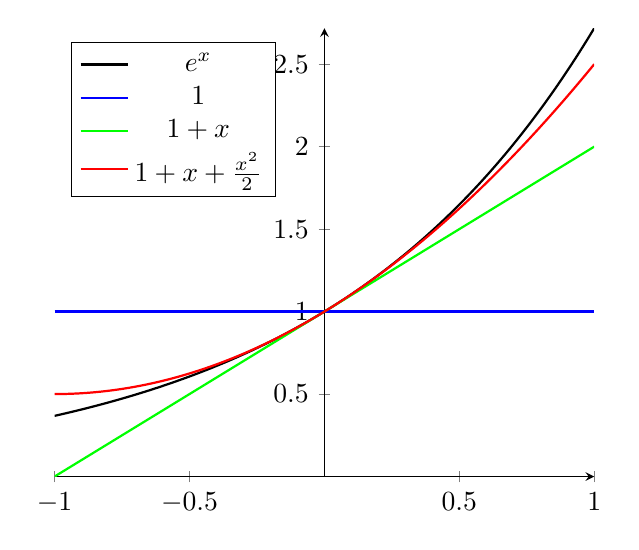
\begin{tikzpicture}
   \begin{axis}[
       axis y line = middle,
       axis x line = middle,
       samples     = 200,
       domain      = -1:1,
       unbounded coords=jump,
       legend pos=north west
     ]
    \addplot[black, thick, mark=none] {exp(x)};
	\addplot[blue, thick, mark=none] {1};     
    \addplot[green, thick, mark=none] {1+x};   
	 \addplot[red, thick, mark=none] {1+x+0.5*x^2};   
	 \addlegendentry{$e^x$}
	 \addlegendentry{$1$}
	 \addlegendentry{$1+x$}
	\addlegendentry{$1+x+\frac{x^2}{2}$}	
   \end{axis}
\end{tikzpicture}
La fonction exponentielle, $x\mapsto e^x$ en bleue, et les fonctions sommes partielles $x\mapsto \sum_{k=0}^{n} \frac{x^k}{k!}$ pour différents valeurs de $n$. On observe la convergence de la fonction somme partielle vers la fonction exponentielle.
}
    \end{minipage}
\end{Exemple}
\begin{Exemple}[Série géométrique] 
Soit  $x\in ]-1,1[$.\\
Par passage à la limite dans l'égalité,  $$\frac{1-x^{n+1}}{1-x}=\sum _{k=0}^{n }x^k,$$ 
on obtient que la  somme de la série $\sum x^{n}$ est  :
$$\frac{1}{1-x}=\sum _{n=0}^{\infty }x^{n}=1+x+x^2 + x^3+\cdots .$$
\end{Exemple}
\subsection{Rayon de convergence}
\begin{Definition}[Domaine de convergence]
On appelle \defi{domaine de convergence} l'ensemble de définition de la fonction $z \mapsto \sum\limits_{n=0}^{+\infty} a_n z^n.$
\end{Definition}
\begin{Exemple}[Série géométrique] 
Le domaine de convergence de la série géométrique $\sum x^{n}$ est $]-1,1[$.\\
\end{Exemple}
 
\begin{Lemme}[Lemme d'Abel]
Soit $\sum a_n z^n$ une série entière et $z_0\in \C$ telle que la suite numérique $(a_n z_0^n)_{n\in \N }$ soit bornée.
Alors:
\begin{enumerate}
\item
  La série numérique $\sum a_n z^n$ converge absolument pour tout $z\in \C$ tel que $|z| < |z_0|$.
\item
  Plus précisément, la série de fonctions $\sum a_n z^n$ converge normalement sur $\{z\in \C:|z|\leq r\}$ dès que $0 \leq r < |z_0|$.
\end{enumerate}
\end{Lemme}
\begin{Demonstration}
Fixons $|z|< |z_{0}|$.\\
$$ \forall n\in \N: \quad |a_{n}\,z^{n}|=\left|a_{n}\,z_{0}^{n}\right|\left|\frac {z}{z_{0}}\right|^{n}.$$
Par hypothèse, le premier des facteurs de ce produit est borné, le second forme une série géométrique de raison strictement inférieure à 1. Par comparaison de séries à termes positifs, la série numérique $\sum a_n z^n$ converge absolument.\\
La démonstration pour la convergence normale est identique ($|a_{n}\,z^{n}|\leq |a_{n}\,r^{n}|=\left|a_{n}\,z_{0}^{n}\right|\left|\frac {r}{z_{0}}\right|^{n}$). 
\end{Demonstration}

\begin{Remarque} Il n'y a pas toujours convergence normale (ni uniforme) sur $\{z\in \C:|z|<|z_0|\}$.
\end{Remarque}
\begin{Lemme}
Soit $\sum a_n z^n$ une série entière et $z_0\in \C$ telle que la suite numérique $(a_n z_0^n)_{n\in \N }$ ne soit pas bornée.
Alors la série numérique $\sum a_n z^n$ diverge grossièrement pour tout $z\in \C$ tel que $|z| \geq |z_0|$.
\end{Lemme}
\begin{Demonstration}
Fixons $|z|\geq  |z_{0}|$.\\
$$ \forall n\in \N: \quad |a_{n}\,z^{n}|=\left|a_{n}\,z_{0}^{n}\right|\left|\frac {z}{z_{0}}\right|^{n}\geq\left|a_{n}\,z_{0}^{n}\right|\xrightarrow[n\to\infty]{}\infty\text{ car }(a_n z_0^n)_{n\in \N }\text{ n'est pas bornée}.$$
Le terme général de la série ne converge  pas vers 0, donc la série numérique $\sum a_n z^n$ diverge grossièrement.
\end{Demonstration}
Si on note $R$, la borne supérieur des rayons telle que la suite $(|a_n| r^n)_{n\in\N}$ est bornée, alors 
\begin{itemize}
\item la série converge si le module du complexe $z$  est  strictement inférieur à $R$ d'après le premier lemme,
\item la série diverge  si le module du complexe $z$  est  strictement supérieur à $R$ d'après le second lemme.
\end{itemize}
Donc la "forme" géométrique du disque de convergence est un disque.
\begin{DefinitionProposition}[Rayon de convergence]
Soit $\sum a_n z^n$ une série entière.\\
Le \defi{rayon de convergence} $R\in \R \cup \{+\infty\}$
de la série entière $\sum a_n z^n$ est défini par
$$
  R = \sup \, \Bigl\{ \, r>0 \text{ tel que la suite de terme général } |a_n| r^n \text{ est bornée} \, \Bigr\}.$$
\begin{itemize}
\item Si $|z_0| < R$, la série numérique $\sum _n a_n z_0^n$ converge absolument.
\item Si $|z_0| > R$, la série numérique $\sum _n a_n z_0^n$ diverge grossièrement; plus précisément, la suite $(a_n z_0^n)_{n\in \N }$ n'est pas bornée.
\item Si $|z_0| = R$, la série peut ou non converger.
\end{itemize}
\begin{center}
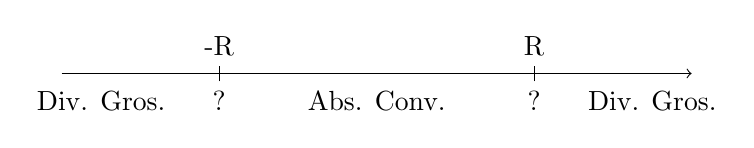
\begin{tikzpicture}[scale=1]
  \draw[->]  (-4,0) -- (4,0) node[right] {$\R$} ;
  \draw[-] (-2,-0.1) node[below] {?}  -- (-2,0.1) node[above] {-R} ;
  \draw (0,-0.1) node[below] {Abs. Conv.} ;
  \draw[-] (2,-0.1) node[below] {?} -- (2,0.1) node[above] {R} ;
  \draw (-3.5,-0.1) node[below] {Div. Gros.} ;
  \draw (3.5,-0.1) node[below] {Div. Gros.} ;			
\end{tikzpicture}\\
Disque de convergence d'une série entière dans le cas réelle
\end{center}


\begin{center}
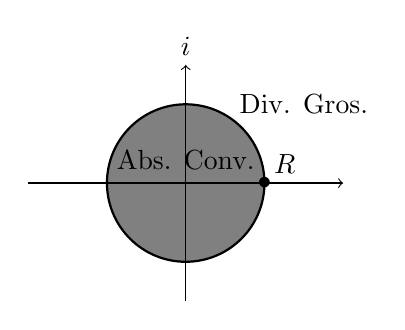
\begin{tikzpicture}[scale=1]
  \filldraw[thick,fill=gray] (0,0) circle (1) ;
  \draw[->] (-2,0) -- (2,0) node[right] {$\R$} ;
  \draw[->] (0,-1.5) -- (0,1.5)node[above] {$i\R$} ;
  \draw (-0,0.3) node {Abs. Conv.};
  \draw (1,0) node {$\bullet$} node[above right] {$R$} ;
  \draw (1.5,1) node {Div. Gros.};
\end{tikzpicture}\\
Disque de convergence d'une série entière dans le cas complexe
\end{center}
\end{DefinitionProposition}





\begin{Demonstration}
Soit $\sum a_n z^n$ une série entière de rayon de convergence $R$.\\
Soit $z \in \C$ fixé.
\begin{itemize}
\item Si $|z | < R$ alors il existe $ r\in\R^+$ tel que $|z | < r < R.$
Comme $(a_n r^n)_{n\in \N}$ est bornée, d'après le lemme d'Abel, la série numérique $\sum a_n z^n$ est absolument convergente.
\item Si $|z | > R$ alors la suite $(a_n z^n)_{n\in \N}$ n'est pas bornée donc ne converge pas vers 0.
Ainsi, la série numérique $\sum a_n z^n$ diverge grossièrement.
\end{itemize}

\end{Demonstration}

\begin{Definition}[Disque ouvert de convergence]
Soit $\sum a_n z^n$ une série entière de rayon de convergence $R$.
\begin{itemize}
\item
  On appelle \defi{intervalle ouvert de convergence} de la série entière $\sum a_n x^n $ à variable réelle l'intervalle
  \[ ]-R,R[. \]
\item
  On appelle \defi{disque ouvert de convergence} de la série entière $\sum a_n z^n$ à variable complexe l'ensemble
  \[ \{z\in \C :|z|<R\}. \]
\item
  On appelle \defi{cercle d'incertitude}
  (et parfois aussi, malheureusement, cercle de convergence)
  de la série entière $\sum a_n z^n$ l'ensemble
  \[ \{z\in \C:|z|=R\}. \]
\end{itemize}
\end{Definition}


% -----------------------------------------------------------------------------
\section{Détermination du rayon de convergence}

\subsection{Encadrement du rayon de convergence}
Si pour un $z_0$ l'on connait la nature de la série numérique $\sum a_n z_0^n$, on en déduit des informations sur le rayon de convergence.
\begin{Proposition}
Soit $\sum a_n z^n$ une série entière de rayon de convergence $R$ et $z_0 \in \C$.
\begin{itemize}
\item Si la série numérique $\sum a_n z_0^n$ converge, alors $|z_0|\geq  R$.
\item  Si la série numérique $\sum a_n z_0^n$ diverge, alors $|z_0|\leq  R$.
\item  Si la série numérique $\sum a_n z_0^n$ est semi convergente, alors $|z_0|=  R$.
\end{itemize}
\end{Proposition}
\begin{Exemple}
Soit la série entière $\sum_{n>0}\frac{x^n}{n}$.\\
 Si $x=-1$, la série alternée $\sum_{n>0}\frac{(-1)^n}{n}$ est semi-convergente. Donc le rayon de convergence est $R=1$.
\end{Exemple}

\subsection{Utilisation de la règle de d'Alembert}
La règle de d'Alembert relative aux séries numériques à termes strictement positifs nous permet la plupart
du temps de déterminer le rayon de convergence d'une série entière. 
\begin{Exemple}
Soit la série entière $\sum \frac{x^n}{n}$.\\
Soit $x\in \R$ fixé. En posant $u_n=\frac{x^n}{n}$, déterminons la nature de la série numérique  $\sum u_n$.\\
D'après la règle de d'Alembert, on a :
$$ \left| \frac{u_{n+1}}{u_n} \right|=\left|  \frac{\frac{x^{n+1}}{n+1}}{\frac{x^n}{n} }  \right|= |x|\frac{n}{n+1}\xrightarrow[n\to +\infty]{} |x|.$$
Si $|x|<1$ la série numérique converge absolument, donc $R\geq 1$.\\
Si $|x|>1$ la série numérique ne converge pas absolument, donc $R\leq 1$.\\
Finalement, $R=1$.
\end{Exemple}

\begin{Exemple}[$\sum a_n x^{\alpha n}$]
Soit la série entière $\sum \frac{x^{2n}}{2^n+1}$.\\
Soit $x\in \R$ fixé.  En posant $u_n=\frac{x^{2n}}{2^n+1}$, déterminons la nature de la série numérique  $\sum u_n$.\\
D'après la règle de d'Alembert,, on a :
$$ \left| \frac{u_{n+1}}{u_n} \right|=\left|  \frac{\frac{x^{2(n+1)}}{2 ^{n+1}+1}}{\frac{x^{2n}}{2^n+1}}  \right|= |x^2|\frac{2^n+1}{2 ^{n+1}+1}\xrightarrow[n\to +\infty]{} \frac{|x|^2}{2}.$$
Si $ \frac{|x|^2}{2}<1$, soit $|x|<\sqrt{2}$, la série numérique converge absolument, donc $R\geq \sqrt{2}$.\\
Si  $ \frac{|x|^2}{2}>1$, soit $|x|>\sqrt{2}$, la série numérique ne converge pas absolument, donc $R\leq \sqrt{2}$.\\
Finalement, $R=\sqrt{2}$.
\end{Exemple}

\subsection{Utilisation de la règle de comparaison}

\begin{Proposition}
Soit $\sum a_n z^n$ et $\sum b_n z^n$ deux séries entières de rayons de convergence
respectivement $R_a$ et $R_b$.
\begin{enumerate}
\item
  Si $|a_n| \leq  |b_n| $ à partir d'un certain rang, alors $R_a\geq R_b$.
\item
  Si $|a_n| = o \left(  |b_n| \right)$   quand $n\to+\infty $, alors $R_a\geq R_b$.
\item
  Si $|a_n| = O \left(  |b_n| \right)$   quand $n\to+\infty $, alors $R_a\geq R_b$.
\item
  S'il existe  $K>0$ tel que $|a_n| \sim K  |b_n|$ quand $n\to+\infty $, alors $R_a = R_b$.
\end{enumerate}
\end{Proposition}
\begin{Demonstration}
Démontrons uniquement la première proposition.\\
Soit $|z|<R_b$ fixé. La série numérique $\sum |b_n z^n|$ est donc convergente. Comme $|a_n| \leq  |b_n| $ à partir d'un certain rang, on a 
$|a_n z^n| \leq  |b_n z^n| $. Cela implique que la série numérique $\sum |a_n z^n|$ est  convergente. En conclusion, $R_a\geq R_b$.
\end{Demonstration}
\begin{Exemple}
Déterminer une borne du rayon de convergence de la série $\sum \sin(n)z^n$.\\
Comme $|\sin(n)|\leq 1$ pour tout $n\in \N$, le rayon de convergence est supérieur ou égale à 1, rayon de convergence de $\sum z^n$. 
\end{Exemple}
\begin{Exemple}
Déterminer le rayon de convergence de la série $\sum \ln(1+1/n)z^n$.\\
Comme $|\ln(1+1/n)|\sim 1/n$, le rayon de convergence est égale à 1, rayon de convergence de $\sum \frac{z^n}{n}$. 
\end{Exemple}
\subsection{Série entière de la forme $\sum n^\alpha a_n z^n$}
\begin{Proposition}
Soit $\alpha\in\R$.\\
Les séries entières $\sum a_n z^n$ et $\sum n^\alpha a_n z^n$ ont même rayon de convergence.
\end{Proposition}
\begin{Demonstration}
Soit $R$ et $R'$ les rayons de convergences des séries $\sum a_n z^n$ et $\sum n^\alpha a_n z^n$ respectivement.\\
On suppose $\alpha\geq 0.$
\begin{itemize}
\item Comme $|a_n|\leq |n^\alpha a_n|$, d'après la règle de comparaison, $R\geq R'$.
\item Soit $|z|<R$ fixé. Montrons que la série numérique  $\sum n^\alpha a_n z^n$ converge absolument.\\
Soit $r \in \R$ tel que $ |z|<r<R$.\\
On a :
$$ |n^\alpha a_n z^n| = |n^\alpha  \frac{z^n}{r^n}| | a_n r^n| \leq M | a_n r^n| \text{ car }  
|n^\alpha  \frac{z^n}{r^n}|\xrightarrow[n\to +\infty]{}0.$$
Comme la série numérique  $\sum | a_n r^n|$ converge puisque $|r|<R$, la série numérique  $\sum |n^\alpha a_n z^n|$ converge par règle de comparaison. En conclusion $R'\geq R$.
\end{itemize}
Pour $\alpha\leq 0$, il faut reprendre cette preuve en inversant l'ordre.
\end{Demonstration}
\begin{Exemple}
Le rayon de convergence de la série $\sum n^{2019}  z^n$ est égale au rayon de convergence de $\sum  z^n$, soit 1. 
\end{Exemple}

% -----------------------------------------------------------------------------
\section{Opérations sur les séries entières}

\subsection{Combinaison linéaire}

\begin{Proposition}
Soit $\sum a_n z^n$ et $\sum b_n z^n$ deux séries entières de rayon de convergence respectif $R_a$ et $R_b$.
\begin{enumerate}
\item $\sum(a_n+b_n)z^n$ est une série entière de rayon de convergence $R$ avec $R = \min( R_a ,R_b )$  si $R_a \neq R_b$
ou $R \geq R_a$ si $R_a = R_b$. De plus, pour $|z|<R$, sa somme est égale à :
$$\sum_{n=0}^{+\infty}(a_n+b_n)z^n = \sum_{n=0}^{+\infty}a_nz^n +\sum_{n=0}^{+\infty}b_n z^n.$$ 
\item $\sum \alpha a_n z^n$ est une série entière de rayon de convergence $R_a$ si $\alpha\neq 0$ et $+\infty$ si $\alpha= 0$. De plus, pour $|z|<R$, sa somme est égale à :
$$\sum_{n=0}^{+\infty}\lambda a_nz^n = \lambda \sum_{n=0}^{+\infty}a_nz^n.$$ 
\end{enumerate}
\end{Proposition}

\begin{Demonstration}[1.]

Ce schéma permet de guider la preuve.\\
\begin{center}
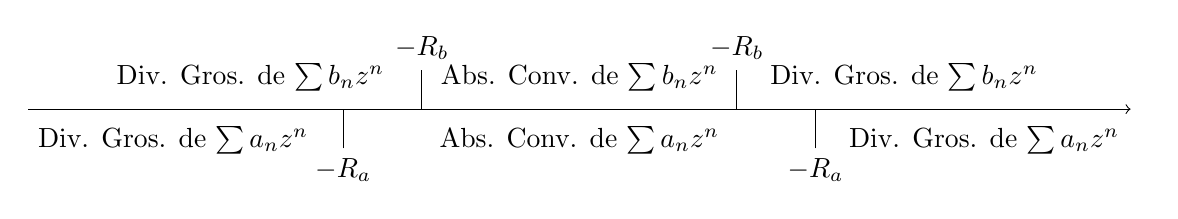
\begin{tikzpicture}[scale=1]
  \draw[->]  (-7,0) -- (7,0) node[right] {$\R$} ;
  \draw[-] (-3,-0.5) node[below ] {$-R_a$}  -- (-3,0);
  \draw[-] (3,-0.5) node[below] {$-R_a$} -- (3,0)  ;
  \draw (0,-0.1) node[below] {Abs. Conv. de $\sum a_n z^n$ } ;
  \draw (-7,-0.1) node[below right] {Div. Gros. de $\sum a_n z^n$} ;
  \draw (3.3,-0.1) node[below right] {Div. Gros. de $\sum a_n z^n$} ;	
  
    \draw[-] (-2,0)  -- (-2,0.5)  node[above] {$-R_b$};
    \draw[-] (2,0)  -- (2,0.5)  node[above] {$-R_b$};	
      \draw (0,0.1) node[above] {Abs. Conv. de $\sum b_n z^n$ } ;
  \draw (-6,0.1) node[above right] {Div. Gros. de $\sum b_n z^n$} ;
  \draw (2.3,0.1) node[above right] {Div. Gros. de $\sum b_n z^n$} ;			
\end{tikzpicture}\\
Les rayons de convergence dans le cas réelle
\end{center}
\begin{itemize}
\item Cas $R_a \neq R_b$ : supposons sans perte de généralité que $R_a < R_b$.\\
\begin{itemize}
\item Soit $|z | < R_a$ fixé d'où $|z | < R_b$. Les deux séries numériques $\sum a_n z^n$ et $\sum b_n z^n$ converge absolument. Donc la série numérique  $\sum(a_n+b_n)z^n$ converge absolument. D'où $R\geq R_a$.
\item  Soit $R_a<|z | <R_b $. La série numérique $\sum a_n z^n$ diverge et la série numérique $\sum b_n z^n$ converge. Donc la série numérique  $\sum(a_n+b_n)z^n$ diverge. D'où $R\leq R_a$.
\end{itemize}
Finalement $R\geq R_a$.
\item Cas $R_a = R_b$ :
\begin{itemize}
\item Soit $|z | < R_a=R_b$ fixé. Les deux séries numériques $\sum a_n z^n$ et $\sum b_n z^n$ converge absolument. Donc la série numérique  $\sum(a_n+b_n)z^n$ converge absolument. D'où $R\geq R_a$.
\item  Soit $|z | > R_a=R_b$ fixé. Les deux séries numériques $\sum a_n z^n$ et $\sum b_n z^n$ divergent. Donc on ne peut rien conclure sur la convergence de la série  $\sum(a_n+b_n)z^n$. 
\end{itemize}
Finalement $R\geq R_a$.
\end{itemize}
\end{Demonstration}
\begin{Exemple}[Rayon de convergence]
\begin{enumerate}
\item $\sum z^n$ et $\sum nz^n$ sont de rayon 1 et leur série entière somme  $\sum (1+n)z^n$ est de rayon 1.
\item $\sum z^n$ et $\sum (2^{-n}-1)z^n$ sont de rayon 1 et leur série entière somme  $\sum (1+n)z^n$ est de rayon 2.
\item $\sum z^n$ et $\sum -z^n$ sont de rayon 1 et leur série entière somme  $\sum 0z^n$ est de rayon $\infty$.
\end{enumerate} 
\end{Exemple}
\begin{Exemple}[Déterminer la somme]
Soit la série entière $\sum (1+\frac{1}{n!})x^n$. \\
Comme $\sum x^n$ est de rayon 1 et  $\sum \frac{x^n}{n!}$ de rayon $\infty$, le rayon de $\sum (1+\frac{1}{n!})x^n$ est 1.\\
Soit $x\in ]-1,1[$ .
$$ \sum_{n=0}^{+\infty} (\frac{1}{n!}+1)x^n= \sum_{n=0}^{+\infty} \frac{x^n}{n!}+ \sum_{n=0}^{+\infty} x^n=e^x+\frac{1}{1-x}.$$
\end{Exemple}
\subsection{Produit de Cauchy}

\begin{Proposition}
Soit $\sum a_n z^n$ et $\sum b_n z^n$ deux séries entières de rayon de convergence respectif $R_a$ et $R_b$.\\
Le \defi{produit de Cauchy} $\sum c_n z^n$  avec $c_n = \sum_{k=0}^n a_k b_{n?k}$ est une série entière de rayon de convergence $R$ avec $R \geq \min( R_a ,R_b )$. De plus, pour $|z|<R$, sa somme est égale à :
$$\sum_{n=0}^{+\infty}c_n z^n = \left(\sum_{n=0}^{+\infty}a_nz^n\right) \times \left(\sum_{n=0}^{+\infty}b_n z^n\right).$$
\end{Proposition}
\begin{Demonstration}
Soit $|z| < \min(R_a,R_b)$. Soit la série numérique $\sum w_n$ produit de Cauchy des séries numériques  $\sum a_n z^n$ et $\sum b_n z^n$. On a :
$$\forall n \in \N : \quad w_n = \sum_{k=0}^n a_k z^k b_{n-k} z^{n-k}=\left(\sum_{k=0}^n a_k  b_{n-k}\right) z^{n}=c_n z^n$$
Comme $\sum a_n z^n$ et $\sum b_n z^n$ sont absolument convergentes, la série numérique $\sum w_n$ est absolument convergente , soit  $R \geq \min( R_a ,R_b )$  et :
 $$\sum_{n=0}^{+\infty}c_n z^n = \left(\sum_{n=0}^{+\infty}a_nz^n\right) \times \left(\sum_{n=0}^{+\infty}b_n z^n\right).$$
\end{Demonstration}
\begin{Exemple}
Le produit de Cauchy de la série géométrique avec elle-même a un rayon égale à 1. De plus, pour tout $|x|<1$, on a :
$$\frac{1}{(1-x)^2}= \left(\sum_{n=0}^{+\infty} x^n\right)^2 =\sum_{n=0}^{+\infty} \left(\sum_{k=0}^n 1\right)x^n =  \sum_{n=0}^{+\infty}(n+1) x^n.$$

\end{Exemple}

\begin{Exemple}
Le produit de Cauchy de la série exponentielle et de la série géométrique a un rayon égale à 1. De plus, pour tout $|x|<1$, on a :
$$\frac{e^x}{1-x}= \left(\sum_{n=0}^{+\infty} \frac{x^n}{n!}\right) \times \left(\sum_{n=0}^{+\infty} x^n\right)=\sum_{n=0}^{+\infty} \left(\sum_{k=0}^n\frac{1}{k!}\right)x^n .$$
\end{Exemple}

% -----------------------------------------------------------------------------
\section{Propriétés de la somme}
La régularité des séries entières est étudiée uniquement dans le cas d'une  variable réelle.\\
Soit $\sum a_n x^n $ une série entière réelle de rayon de convergence $R$ et de somme $f:x\mapsto \sum\limits_{n=0}^{+\infty}\ln(n)x^n$.
\begin{Theoreme}[continuité]
$f$ est continue sur l'intervalle de convergence $]-R,R[$.
\end{Theoreme}
\begin{Exemple}
$f:x\mapsto\sum\limits_{n=0}^{+\infty} \ln(n) x^{n}$ est continue sur $]-R,R[$.
\end{Exemple}

\begin{Theoreme}[dérivation terme à terme]
$\sum n a_n x^{n-1}$ est une série entière de rayon de convergence $R$.\\
$f$ est dérivable sur $]-1,1[$ et sa fonction dérivée  sur $]-R,R[$, $f'$, est égale à:
$$\forall x\in ]R,R[:f'(x)=\left(\sum_{n=0}^{+\infty} a_n x^{n}\right)'{\color{red}{=}}\sum_{n=0}^{+\infty} \left(a_n x^{n}\right)'= \sum_{n=0}^{+\infty}n a_n x^{n-1}.$$
\end{Theoreme}
\begin{Exemple}[dérivation de la série géométrique]
Soit la série géométrique $\sum  x^{n}$. On a
$$\forall x\in]-1,1[:\quad \frac{1}{1-x}=\sum_{n=0}^{+\infty}x^n.$$
Par le théorème de dérivation terme à terme, on obtient :
$$\forall x\in]-1,1[:\quad \frac{1}{(1-x)^2}=\sum_{n=0}^{+\infty}nx^{n-1}.$$
Donc la somme de la série entière $\sum_{n}nx^{n-1}$ est la fonction $x\mapsto \frac{1}{(1-x)^2}$.
\end{Exemple}
\begin{Theoreme}[intégration terme à terme]
$\sum n \frac{a_n}{n+1} x^{n+1}$ est une série entière de rayon de convergence $R$.\\
Soit $F$ une primitive de $f$. On a 
$$\forall x\in ]R,R[:F(x)-F(0)=\int_0^x \left( \sum_{n=0}^{+\infty} a_n t^{n}\right) dt{\color{red}{=}}\sum_{n=0}^{+\infty} \int_{0}^{x} a_n t^{n}dt= \sum_{n=0}^{+\infty}\frac{a_n}{n+1} x^{n+1}.$$
\end{Theoreme}
\begin{Exemple}[intégration de la série géométrique]
Soit la série géométrique $\sum  x^{n}$. On a
$$\forall x\in]-1,1[:\quad \frac{1}{1-x}=\sum_{n=0}^{+\infty}x^n.$$
Par le théorème d'intégration terme à terme, on obtient :
$$\forall x\in]-1,1[:\quad -\ln(1-x)=\sum_{n=0}^{+\infty}\frac{x^{n+1}}{n+1}.$$
Donc la somme de la série entière $\sum_{n}\frac{x^{n+1}}{n+1}$ est la fonction $x\mapsto -\ln(1-x)$.
\end{Exemple}

% -----------------------------------------------------------------------------
\section{Développements en séries entières}
\subsection{Généralités}
\begin{Definition}[fonction développable en série entière]
On dit que $f$ est \defi{développable en série entière} sur $]-r,r[$ (au voisinage de $0$)
si il existe une série entière $\sum a_n x^n $ de rayon de convergence $R\geq r $ telle que
\[ \forall x\in ]-r ,r [,\quad f(x) = \sum_{n=0}^{+\infty} a_n x^n. \]
\end{Definition}
\begin{Exemple}[série géométrique]
On a :
$$ \forall x\in ]-1,1[:\quad  \frac{1-x^{N+1}}{1-x}=\sum_{n=0}^N x^n.$$
Par passage à la limite, on obtient :
$$ \forall x\in ]-1,1[:\quad  \frac{1}{1-x}=\sum_{n=0}^{+\infty}x^n.$$
Donc la fonction $x\mapsto  \frac{1}{1-x}$  est développable en série entière.
\end{Exemple}
\begin{Theoreme}[condition nécessaire]
Si $f$ admet un développement en série entière sur $]-r, r [$ alors $f$ est de classe $\mathcal{C}^{+\infty}$ sur $]-r, r [$, son
développement en série entière est unique et est donné par sa \defi{série de Taylor} :
$$\forall x\in ]-r ,r [,\quad f(x) = \sum_{n=0}^{+\infty} \frac{f^{(n)}(0)}{n!} x^n. $$ 
\end{Theoreme}
\begin{Remarque}
La réciproque du théorème est fausse.
Il se peut qu'une fonction $f$ soit de classe $\mathcal{C}^{+\infty}$ sur $]-r, r [$ sans que $f$ soit  développable en série entière. Considérons, par exemple, la fonction $f$ définie par :
$$\Fonction{f}{\R}{\R}{x}{\begin{cases}e^{-\frac{1}{x^2}}&\text{ si }x\neq 0\\ 0 &\text{ si }x= 0 \end{cases} }.$$
\begin{itemize}
\item L'application $f$ est  $\mathcal{C}^{\infty}$ sur $\R^*$ et on montre, par récurrence sur $n$, que, pour tout $n\in \N$, il existe $P_n\in \R[X]$ tel que :
$$\forall x\in \R^*,\quad, f^{(n)}(x)=\frac{P_n(x)}{x^{3n}}  e^{-\frac{1}{x^2}}.$$ 
Une application répétée du théorème limite de la dérivée permet de déduire que  $f$ est de classe $\mathcal{C}^{+\infty}$ sur $\R$ et :
$$ \forall n\in \N,\quad f^{(n)}(0)=0.$$
\item Si $f$ était développement en série entière, il existerait $r$ tel que :
$$\forall x \in ]-r,r[,\quad f(x) = \sum_{n=0}^{+\infty} \frac{f^{(n)}(0)}{n!} x^n\overbrace{=}^{f^{(n)}(0)=0}0,$$
ce qui est impossible puisque $f$ ne s'annule qu'en 0.
\end{itemize}

\end{Remarque}
\begin{Corollaire}[unicité du développement en série entière]
Si $$\forall x \in] - r, r [,\quad \sum_{n=0}^{+\infty} a_n x^n= \sum_{n=0}^{+\infty} b_n x^n,$$alors on a : $$\forall n\in \N,\quad a_n=b_n.$$
\end{Corollaire}
\begin{Remarque}
Cette égalité $0=\sum_{n=0}^{+\infty} 0 x^n$ est importante.
\end{Remarque}

\begin{Corollaire}[développement limitée]
Si $$\forall x \in] - r, r [,\quad f(x)=\sum_{n=0}^{+\infty} a_n x^n$$alors on a : $$\forall x \in] - r, r [,\quad f(x)=\sum_{n=0}^N a_n x^n+o(x^N).$$
\end{Corollaire}
\subsection{Méthodes pratiques}
\begin{enumerate}
\item Utilisation des opérations somme et produit.\\
\begin{Exemple} Déterminer le développement en série entière de $f : x \mapsto \frac{1}{1-x} + 2e^x.$
$$\forall x\in]-1,1[:\quad f(x)=\sum_{n=0}^{+\infty} x^n +2\sum_{n=0}^{+\infty} \frac{x^n}{n!}=\sum_{n=0}^{+\infty} (1+\frac{2}{n!})x^n.$$
\end{Exemple}
\item Changement de variable.\\
\begin{Exemple} Déterminer le développement en série entière de $f : x \mapsto \frac{1}{a-x} .$
$$\forall x\in]-a,a[:\quad f(x)=\frac{1}{a}\frac{1}{1-\frac x a}\overbrace{=}^{\text{en posant }y=\frac x a \text{ avec } \frac{1}{1-y}=\sum\limits_{n=0}^{+\infty} y^n} \frac{1}{a}\sum_{n=0}^{+\infty} \left(\frac{x}{a}\right)^n =  \sum_{n=0}^{+\infty} \frac{x^n}{a^{n+1}}  .$$
\end{Exemple}
\item Décomposition en éléments simples d'une fraction rationnelle.\\
\begin{Exemple} Déterminer le développement en série entière de $f : x \mapsto \frac{1}{x^2-3x+2} .$
$$\forall x\in]-1,1[:\quad f(x)= \frac{1}{x^2-3x+2} =\frac{1}{1-x}-\frac{1}{2-x}= \sum_{n=0}^{+\infty} (1-\frac{1}{2^{n+1}})x^n .$$
\end{Exemple}

\item  Dérivation et intégration terme à terme.
\begin{Exemple} Déterminer le développement en série entière de $f : x \mapsto \ln(1-x).$\\
Soit $x\in]-1,1[$.
$$\begin{aligned} 
 \ln(1-x) =&-\int_0^x \frac{1}{1-t}dt\\
  =& \int_0^x \sum_{n=0}^{+\infty} t^n dt \\
 =& \sum_{n=0}^{+\infty} \int_0^x t^n dt \text{ (théorème d'intégration terme à terme)}\\
 =&\ \sum_{n=0}^{+\infty} \frac{x^{n+1}}{n+1}.
 \end{aligned}$$
\end{Exemple}

\item Utilisation d'une équation différentielle.
\begin{Exemple} Déterminer le développement en série entière de $f : x \mapsto \cos(x).$. \\
La fonction $f$ est l'unique solution du problème de Cauchy de l'équation différentielle :
$$y''=-y, \quad  y(0)=1, y'(0)=0, \text{ sur } \R\quad (E).$$ 
Supposons qu'il existe une solution de $(E)$ sous forme de série entière $\sum_{n=0}^{+\infty} a_nx^n$ de somme $f$. Soit $x\in \R$. On a :
$$\begin{aligned} 
 f''(x)=&\sum_{n=0}^{+\infty} n(n-1) a_nx^{n-2}\\
  =& \sum_{n=2}^{+\infty} n(n-1) a_n x^{n-2} \text{ (les deux premiers termes sont nuls)}\\
 =&\sum_{n=0}^{+\infty} (n+2)(n+1) a_{n+2}x^{n} \text{ (translation d'indice)}.
 \end{aligned}$$
Comme $f''=-f$, par identification, on obtient : 
$$\forall n\in\N : \quad   (n+2)(n+1) a_{n+2} =-a_n.$$
On a $f(0)=a_0$ et $f'(0)=a_1$. D'après les conditions initiales  $f(0)=1$ et $f'(0)=0$, d'où $a_0=1$ et $a_1=0$. Par récurrence, on démontre que :
$$\forall n\in\N : \quad   a_{2n} =\frac{(-1)^n}{(2n)!}\text{ et }  a_{2n+1}=0.$$
Finalement, on obtient :
$$\forall x \in \R,\quad \cos(x)=\sum_{n=0}^{+\infty}  \frac{(-1)^n}{(2n!}x^ {2n}.$$
\end{Exemple}
\end{enumerate}

% -----------------------------------------------------------------------------
\section{Développements en série entière usuels}

Dans l'exemple introductif du chapitre, la fonction $\exp$ est l'unique solution du problème de Cauchy $y' = y$ avec $y (0) = 1$. On prolonge $\exp$ à $\C$.
\begin{Definition}[Exponentielle complexe]
La série entière $\sum_{n=0}^{+\infty} \frac{z^n}{n!}$ est de rayon de convergence infini. Sa somme est appelé l'\defi{exponentielle complexe}. On a ainsi :
$$\forall z\in \C,\quad \exp(z)=\sum_{n=0}^{+\infty}  \frac{z^n}{n!}.$$
On note $e^z=\exp(z).$
\end{Definition}
\begin{Proposition}
$$\forall z,z'\in \C:\quad e^{z+z'}=e^z.e^{z'}.$$
\end{Proposition}

\begin{Demonstration}
La démonstration est faite dans le chapitre sur les séries numériques à la section produit de Cauchy.
\end{Demonstration}
On a aussi :\\
\begin{tabular}{l|ll}
$R=\infty$ & $\forall x \in\R:$& $\cos x  = \sum\limits_{n=0}^{+\infty} \frac{(-1)^n}{(2n)!} \, x^{2n}$\\ \hline
$R=\infty$ & $\forall x \in\R:$&$\sin x  =  \sum\limits_{n=0}^{+\infty} \frac{(-1)^n}{(2n+1)!} \, x^{2n+1}$\\ \hline
$R=\infty$ & $\forall x \in\R: $&$\text{ch} x =  \sum\limits_{n=0}^{+\infty} \frac{1}{(2n)!} \, x^{2n}$\\ \hline
$R=\infty$ & $\forall x \in\R:$&$ \text{sh} x =  \sum\limits_{n=0}^{+\infty} \frac{1}{(2n+1)!} \, x^{2n+1}$\\ \hline
$R=1$ & $\forall x \in]-1,1[:$&$ \frac{1}{1+x} = \sum\limits_{n=0}^{+\infty} (-1)^n \, x^{n}$\\ \hline
$R=1$ & $\forall x \in]-1,1[:$&$ \ln(1+x) =  \sum\limits_{n=0}^{+\infty} \frac{(-1)^{n+1}}{n} \, x^{n}$
\end{tabular}


\end{document}
